% A LaTeX (non-official) template for ISAE projects reports
% Copyright (C) 2014 Damien Roque
% Version: 0.2
% Author: Damien Roque <damien.roque_AT_isae.fr>

\documentclass[a4paper,12pt]{book}
%\documentclass[french]{article}
\usepackage[utf8]{inputenc}
\usepackage[T1]{fontenc}
%\usepackage[french]{babel} % If you write in French
%\usepackage[english]{babel} % If you write in English
\usepackage[english,francais,french, frenchb]{babel}

\usepackage{a4wide}
\usepackage{graphicx}
\graphicspath{{images/}}
\usepackage{subfig}
\usepackage{tikz}
\usetikzlibrary{shapes,arrows}
\usepackage{pgfplots}
\pgfplotsset{compat=newest}
\pgfplotsset{plot coordinates/math parser=false}
\newlength\figureheight
\newlength\figurewidth
\pgfkeys{/pgf/number format/.cd,
set decimal separator={,\!},
1000 sep={\,},
}
\usepackage{ifthen}
\usepackage{ifpdf}
\ifpdf
\usepackage[pdftex]{hyperref}
\else
\usepackage{hyperref}
\fi
\usepackage{color}
\hypersetup{%
colorlinks=true,
linkcolor=black,
citecolor=black,
urlcolor=black}

\renewcommand{\baselinestretch}{1.05}
\usepackage{fancyhdr}
\pagestyle{fancy}
\fancyfoot{}
\fancyhead[LE,RO]{\bfseries\thepage}
\fancyhead[RE]{\bfseries\nouppercase{\leftmark}}
\fancyhead[LO]{\bfseries\nouppercase{\rightmark}}
\setlength{\headheight}{15pt}

\let\headruleORIG\headrule
\renewcommand{\headrule}{\color{black} \headruleORIG}
\renewcommand{\headrulewidth}{1.0pt}
\usepackage{colortbl}
\arrayrulecolor{black}

\fancypagestyle{plain}{
  \fancyhead{}
  \fancyfoot[C]{\thepage}
  \renewcommand{\headrulewidth}{0pt}
}

\makeatletter
\def\@textbottom{\vskip \z@ \@plus 1pt}
\let\@texttop\relax
\makeatother

\makeatletter
\def\cleardoublepage{\clearpage\if@twoside \ifodd\c@page\else%
  \hbox{}%
  \thispagestyle{empty}%
  \newpage%
  \if@twocolumn\hbox{}\newpage\fi\fi\fi}
\makeatother

\usepackage{amsthm}
\usepackage{amssymb,amsmath,bbm}
\usepackage{array}
\usepackage{bm}
\usepackage{multirow}
\usepackage[footnote]{acronym}

\newcommand*{\SET}[1]  {\ensuremath{\mathbf{#1}}}
\newcommand*{\VEC}[1]  {\ensuremath{\boldsymbol{#1}}}
\newcommand*{\FAM}[1]  {\ensuremath{\boldsymbol{#1}}}
\newcommand*{\MAT}[1]  {\ensuremath{\boldsymbol{#1}}}
\newcommand*{\OP}[1]  {\ensuremath{\mathrm{#1}}}
\newcommand*{\NORM}[1]  {\ensuremath{\left\|#1\right\|}}
\newcommand*{\DPR}[2]  {\ensuremath{\left \langle #1,#2 \right \rangle}}
\newcommand*{\calbf}[1]  {\ensuremath{\boldsymbol{\mathcal{#1}}}}
\newcommand*{\shift}[1]  {\ensuremath{\boldsymbol{#1}}}

\newcommand{\eqdef}{\stackrel{\mathrm{def}}{=}}
\newcommand{\argmax}{\operatornamewithlimits{argmax}}
\newcommand{\argmin}{\operatornamewithlimits{argmin}}
\newcommand{\ud}{\, \mathrm{d}}
\newcommand{\vect}{\text{Vect}}
\newcommand{\sinc}{\ensuremath{\mathrm{sinc}}}
\newcommand{\esp}{\ensuremath{\mathbb{E}}}
\newcommand{\hilbert}{\ensuremath{\mathcal{H}}}
\newcommand{\fourier}{\ensuremath{\mathcal{F}}}
\newcommand{\sgn}{\text{sgn}}
\newcommand{\intTT}{\int_{-T}^{T}}
\newcommand{\intT}{\int_{-\frac{T}{2}}^{\frac{T}{2}}}
\newcommand{\intinf}{\int_{-\infty}^{+\infty}}
\newcommand{\Sh}{\ensuremath{\boldsymbol{S}}}
\newcommand{\C}{\SET{C}}
\newcommand{\R}{\SET{R}}
\newcommand{\Z}{\SET{Z}}
\newcommand{\N}{\SET{N}}
\newcommand{\K}{\SET{K}}
\newcommand{\reel}{\mathcal{R}}
\newcommand{\imag}{\mathcal{I}}
\newcommand{\cmnr}{c_{m,n}^\reel}
\newcommand{\cmni}{c_{m,n}^\imag}
\newcommand{\cnr}{c_{n}^\reel}
\newcommand{\cni}{c_{n}^\imag}
\newcommand{\tproto}{g}
\newcommand{\rproto}{\check{g}}
\newcommand{\LR}{\mathcal{L}_2(\SET{R})}
\newcommand{\LZ}{\ell_2(\SET{Z})}
\newcommand{\LZI}[1]{\ell_2(\SET{#1})}
\newcommand{\LZZ}{\ell_2(\SET{Z}^2)}
\newcommand{\diag}{\operatorname{diag}}
\newcommand{\noise}{z}
\newcommand{\Noise}{Z}
\newcommand{\filtnoise}{\zeta}
\newcommand{\tp}{g}
\newcommand{\rp}{\check{g}}
\newcommand{\TP}{G}
\newcommand{\RP}{\check{G}}
\newcommand{\dmin}{d_{\mathrm{min}}}
\newcommand{\Dmin}{D_{\mathrm{min}}}
\newcommand{\Image}{\ensuremath{\text{Im}}}
\newcommand{\Span}{\ensuremath{\text{Span}}}

\newtheoremstyle{break}
  {11pt}{11pt}%
  {\itshape}{}%
  {\bfseries}{}%
  {\newline}{}%
\theoremstyle{break}

%\theoremstyle{definition}
\newtheorem{definition}{Définition}[chapter]

%\theoremstyle{definition}
\newtheorem{theoreme}{Théorème}[chapter]

%\theoremstyle{remark}
\newtheorem{remarque}{Remarque}[chapter]

%\theoremstyle{plain}
\newtheorem{propriete}{Propriété}[chapter]
\newtheorem{exemple}{Exemple}[chapter]

\parskip=5pt
%\sloppy

\begin{document}

%%%%%%%%%%%%%%%%%%
%%% First page %%%
%%%%%%%%%%%%%%%%%%

\begin{titlepage}
\begin{center}


\includegraphics[width=0.6\textwidth]{logo-lriXu10}\\[1cm]

{\large Master 1 MIAGE,  Agilité des Systèmes d’Information et e-Business de l’Université Paris Nanterre }\\[0.5cm]

{\large Rapport de stage}\\[0.5cm]

% Title
\rule{\linewidth}{0.5mm} \\[0.4cm]
{ \huge \bfseries Application mobile pour système de recommandation d’articles \\[0.4cm] }
\rule{\linewidth}{0.5mm} \\[1.5cm]

% Author and supervisor
\noindent
\begin{minipage}{0.4\textwidth}
  \begin{flushleft} \large
    \emph{Auteurs :}\\
    M. Fabien \textsc{MICHEL}\\
    %M\up{me} Prénom \textsc{Nom}\\
  \end{flushleft}
\end{minipage}%
\begin{minipage}{0.4\textwidth}
  \begin{flushright} \large
    \emph{Encadrants :} \\
    Dr.~Bich-Lien \textsc{Doan}\\
    M.~Julien \textsc{Hay}\\
    Dr.~Jean-François \textsc{PRADAT-PEYRE}\\
    
    
  \end{flushright}
\end{minipage}

\vfill

% Bottom of the page
{\large Version 1\\ du\\ \today}

\end{center}
\end{titlepage}

%%%%%%%%%%%%%%%%%%%%%%%%%%%%%
%%% Non-significant pages %%%
%%%%%%%%%%%%%%%%%%%%%%%%%%%%%

\frontmatter

\chapter*{Remerciements}

Je tiens à remercier toutes les personnes qui ont contribué au succès de mon stage et qui m’ont aidé lors de la rédaction de ce rapport. 

Je tiens à remercier vivement mon maitre de stage officieux, M. Julien HAY, pour son accueil, le temps passé ensemble et le partage de son expertise au quotidien. Grâce aussi à sa confiance j'ai pu m'épanouir totalement dans mes missions. Il fut d'une aide précieuse dans les moments les plus délicats. 

Je tiens à remercier vivement M. Alexis JODAR qui m’a accompagné tout au long de cette expérience professionnelle avec beaucoup d'humour, de patience et de pédagogie. 

Je remercie Bich-Lien Doan ainsi que Jean-François PRADAT-PEYRE, pour leurs conseils avisés et sans qui je n'aurai pu réaliser ce stage. 

Enfin, j’adresse mes plus sincères remerciements à ma femme Marjolaine LEVEAU qui m’as soutenu et m’a encouragé comme toujours mais particulièrement pendant cette période de stage. 

 

\clearpage
\tableofcontents

\clearpage
\listoffigures

\clearpage
\chapter*{Liste des sigles et acronymes}
\begin{acronym}[CP-OFDMX] % Give the longest acronym here
\acro{OS}{\emph{Operating System}}
\acro{LRI}{\emph{Laboratoire de Recherche en Informatique}}
\end{acronym}

%%%%%%%%%%%%%%%%%%%%%%%%%%%%%%%%%%%%%%%%%%%%
%%% Content of the report and references %%%
%%%%%%%%%%%%%%%%%%%%%%%%%%%%%%%%%%%%%%%%%%%%

\mainmatter
\pagestyle{fancy}

\cleardoublepage

\chapter*{Introduction}
\addcontentsline{toc}{chapter}{Introduction}
\markboth{Introduction}{Introduction}
\label{chap:introduction}
%\minitoc

Selon une étude de l'Alliance pour les Chiffres de la Presse et des Médias (ACPM) \cite{oneGlobal}. En 2016, les Français ont lu 5,6 titres différents (quotidiens et magazines confondus) chaque mois en moyenne. Ce sont les femmes qui lisent plus de titres que la moyenne tout comme les « ultraconnectés». Les versions papiers représentent 51 \% des lectures contre 49 \% pour les versions numériques dont le pourcentage augmente d'année en année sur la version papier. Cette tendance est particulièrement marquée chez les personnes âgées de 15 à 24 ans privilégient le mobile et dont 55 \% d'entre eux lisent au moins une marque de presse sur mobile. Les marques de presse ont compris qu'il fallait toucher le maximum de personnes sur les applications mobiles dont la tranche des 15-24 ans utilisent le plus, c’est-à-dire les réseaux sociaux. Sur les réseaux sociaux, c'est sur Twitter que les marques de presse sont les plus suivies avec 55 \% des personnes interrogées utilisant régulièrement Twitter suivent une marque de presse suivit par Google+ et Facebook. Si la majorité de ces internautes suivent une marque de presse, c'est pour suivre l'actualité en temps réel à 72 \%, partager les articles avec leurs contacts et trouver des informations qu'ils ne trouvent pas ailleurs.  

Dans le sous-domaine de la recommandation d’articles d’actualités, il existe à ce jour très peu de systèmes permettant aux différentes équipes de recherche de tester leurs algorithmes en temps réel sur des utilisateurs interagissant directement avec le système de recommandation. L'idée de l'application Renewal est née de ce constat mais ne veux pas se cantonner au monde de la recherche. La finalité est d'avoir une application utilisée par un grand nombre d'utilisateur permettant la récolte et l'analyse fine du comportement de chaque  utilisateur. Le but est double, pour les utilisateurs recevoir un feed d'actualité pertinent avec ses gouts et pour les équipes de recherches déterminer l'algorithme de recommandation le plus pertinent.  

Dans le cadre de ma première année de Master MIAGE (Méthodes Informatiques Appliquées à la Gestion des Entreprises à l'Université de Paris Nanterre, j'ai souhaité réaliser un stage me permettant de me former sur le développement d'application mobile en complément de ce qui m'as été dispensé durant ma formation. J'ai effectué ce stage au sein du Laboratoire de Recherche en Informatique du 7 avril au 31 juillet 2018. 

%%% Local Variables: 
%%% mode: latex
%%% TeX-master: "lri-report"
%%% End: 

\chapter{Cadre général}
\label{sec:Cadre général}

\section{Présentation de l’Entreprise}

\subsection{Le LRI}
Le Laboratoire de Recherche en Informatique(LRI) est une unité de recherche de l'Université Paris Sud en partenariat avec le CNRS, le Centre National de la Recherche Scientifique, l'INRIA et Centrale / Supelec. Fondé il y a plus de 35 ans, il compte plus de 250 membres, dont plus de 130 professeurs et membres du personnel et 88 doctorants. Le LRI se compose de neuf groupes de recherche, soutenus par un personnel administratif et technique. Quatre des groupes de recherche sont totalement ou partiellement associés à Inria Saclay Ile de France, ce qui en fait l'un des principaux partenaires du laboratoire. Le laboratoire est situé sur le plateau de Moulon dans ses nouveaux bâtiments connectés Ada Lovelace et Claude Shannon.

Les thèmes de recherche du laboratoire couvrent un large spectre de l'informatique à dominante logicielle et incluent à la fois des aspects fondamentaux et des aspects appliqués : algorithmique, combinatoire, graphes, optimisation discrète et continue, programmation, génie logiciel, vérification et preuves,  parallélisme, calcul à haute performance, grilles, architecture et compilation, réseaux, bases de données, représentation et traitement des connaissances, apprentissage, fouille de données, bioinformatique, interaction homme-machine, etc.  Cette diversité est l'une des forces du laboratoire car elle favorise les recherches aux frontières, là où le potentiel d'innovation est le plus grand.

Le laboratoire participe à un grand nombre de projets nationaux et internationaux, notamment ceux financés par l'Agence National de la Recherche (ANR), par Digiteo et par l'Union européenne (notamment la CCI ICT Labs de l'EIT). Les membres du LRI participent à de nombreux comités éditoriaux de revues internationales et comités de programme de conférences internationales. Le laboratoire a également une très forte activité de publication avec plus de 2000 publications entre début 2008 et mi 2013 ainsi qu'une importante activité de production logicielle et de transfert.

Le LRI fait partie de Digiteo l'un des douze réseaux de recherche créés par le gouvernement français en 2007 et le seul en sciences et technologies de l'information (STIC). Digiteo rassemble sur le plateau de Saclay 1200 chercheurs issus de 23 laboratoires de six instituts nationaux de recherche fondateurs (CNRS, CEA, Inria, Université Paris-Sud, Ecole Polytechnique, Supélec) et de six membres associés (Ecole Centrale Paris, ENS Cachan, Université de Versailles Saint Quentin en Yvelines, Institut Mines-Télécom, Mines ParisTech, ENSTA ParisTech). Le LRI est également partenaire de System@tic Paris-Région, un pôle de compétitivité de classe mondiale regroupant plus de 200 industriels, universitaires et institutionnels dans le domaine des logiciels et systèmes complexes.

Le LRI est fortement impliqué dans les programmes d'Investissements d'Avenir lancés en 2010 par le gouvernement français. Il dirige l'Equipex Digiscope, du Labex Digicosme qui participe à l'IRT SystemX et est très actif dans l'Idex Paris-Saclay qui donnera naissance en 2014 à la nouvelle Université Paris-Saclay: Le LRI joue un rôle important dans la mise en place du futur département STIC dans la continuité de Digiteo et dirige les projets de l'Ecole Doctorale STIC et du Master Informatique de l'Université Paris-Saclay.

\subsection{Chiffres clés}

Le LRI compte plus de 250 membres, dont plus de 112 professeurs permanents, 88 doctorants, 27 ingénieurs, techniciens, personnel administratif. Ses menbres ont durant la période 2010-2014 effectué plus de 2000 publications. Le LRI est un partenaire académique d'envergure international avec des partenarias avec des universités préstigieuse dont notamment l'Université de Tokyo, l'Université de Montréal,  l'Université d'Oxford, l'Université de Californie à Berkeley, l'Université de Vienne Autriche,... L'une des forces du laboratoire est d'avoir des partenaires industriels de choix tels que :  EDF,Thalès,Nokia, Philips, L'oréal, IBM, Schneider, SAP Sirehna qui permettent aux chercheurs d'être connectés avec la réalité industrielle et ses enjeux. 


\subsection{Organisation et l'equipe MODHEL}

Le Laboratoire de Recherche informatique est composé de 9 équipes de recherche. J'ai effectué mon stage au sein de l'équipe Modélisation Hétérogène (MODHEL) dirigé par Frédéric BOULANGER. Chaque équipe de recherche travaille soit sur un logiciel et brevet soit sur une thèses ou une habilitations récentes.

\begin{figure}[htp]
  \centering
  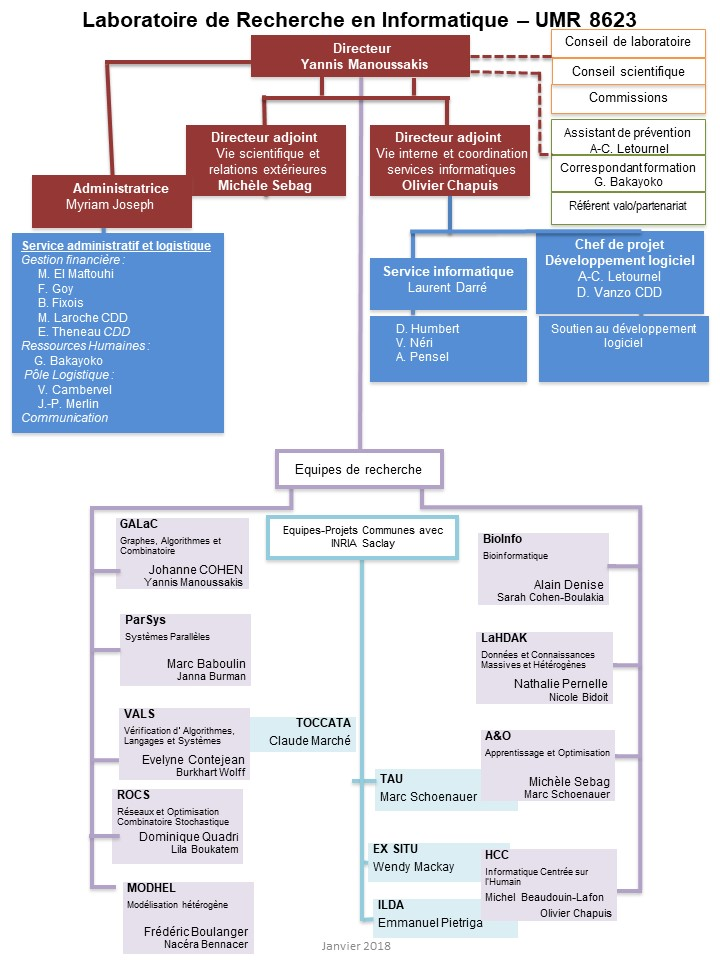
\includegraphics[width=7cm]{images/Orga_LRI}
  \caption{Organigramme du LRI.}
  \label{fig:une-autre-image}
\end{figure}

Mon sujet de stage m’a conduit à travailler sur la thèse de Julien HAY qui s'intitule : "Analyse des réseaux sociaux pour enrichir et segmenter les profils utilisateurs. Cette thèse en préparation à Paris Saclay , dans le cadre de Sciences et Technologies de l'Information et de la Communication , en partenariat avec le LRI au sein de l'équipe de recherche MODHEL et Central Supélec  (établissement de préparation de la thèse) depuis le 20-03-2017. Durant mon stage, mon équipe de travail au sein de l’équipe MODHEL est composé de Julien HAY qui est donc un doctorant mais aussi  mon tuteur de stage et Alexis JODAR un étudiant en 3ième année d’étude au sein de l’école epitech qui va s’occuper du back-end de l’application 


\subsection{Résumé de la thèse de J. HAY}

Le travail de recherche de Julien HAY vise à améliorer et à développer de nouveaux algorithmes de segmentation et d'enrichissement des profils utilisateurs tout en validant leur application dans le cadre de la plateforme industrielle Octopeek. Octopeek est une startup spécialisée en Big Data et Data Science. Dans le cadre de cette thèse, il est prévu de mettre en place des méthodes d'extraction et d'analyse des données internes aux réseaux sociaux mais également issues d'autres sources de données en vue de leur réutilisation dans la plateforme Octopeek. Néanmoins, la réalisation d'un tel système demeure un défi scientifique qui devra prendre en compte le volume de données, le temps d'exécution de la recherche et la sémantique des termes afin de fournir les meilleures réponses. En effet, pour chaque information recherchée, il faudra trouver la méthode, l'algorithme optimisé qui prend en compte la rapidité de calcul, et le scoring associé. A terme il sera amené à implémenter des algorithmes pour une utilisation à la volée et sur plusieurs personnes en parallèle.


\section{Sujet du stage}

\subsection{Missions et enjeux}

L'objectif premier de ce stage est le développement d’une application mobile qui présentera des articles d’actualité aux utilisateurs selon leurs intérêts. L’application devra être multi-plateforme : Android et iOS et devra permettre l’évaluation de différents systèmes de recommandation grâce à des métriques telles que CTR (Click-through rate). Avec l’accord de chaque utilisateur, une analyse précise de leur navigation (géolocalisation, temps de lecture, scroll des articles. . .) et comportement permettra de capturer des éléments de contexte et des retours de pertinence implicites utiles aux algorithmes de recommandation. Chaque utilisateur sera identifié par son profil sur les réseaux sociaux (Facebook, Twitter) ou via une adresse mail. Dans une seconde partie du stage, il est prévu de construire un système de recommandation baseline s’appuyant sur les activités passées de chaque utilisateur, ainsi que sur une base de données d’articles renouvelée en temps réel. Ce travail sera réalisé sous la supervision du doctorant en charge du projet et en collaboration avec un second stagiaire réalisant la partie architecture et récolte de données (notamment pour alimenter la base de données d’articles). 

\subsection{Problématique}

Les recherches dans le domaine des systèmes de recommandation s’appuient la plupart du temps sur des évaluations “offline” qui ne permettent pas d’établir des métriques en phase avec une réelle satisfaction utilisateur. Dans le sous-domaine de la recommandation d’articles d’actualité, il existe à ce jour très peu de systèmes permettant aux différentes équipes de recherche de tester leurs algorithmes en temps réel, i.e. sur des utilisateurs interagissant directement avec le système de recommandation. 


Nous proposons de développer une application mobile qui tentera de contourner ces obstacles et  permettra dans un premier temps, l’évaluation de nos algorithmes de recommandation sur des utilisateurs en contexte et en temps réel. Et permettra, dans un second temps la confrontation de différentes équipes de recherche du domaine.




%%% Local Variables: 
%%% mode: latex
%%% TeX-master: "lri-report"
%%% End: 
\chapter{Plannification et gestion de projet}
\label{sec:Plannification et gestion de projet}

\section{Contexte}

La réalisation de l'application s'est effectuée de façon agile. L'agilité représente un ensemble de méthodes, de process, fortement orienté collaboratif avec une certaine transversalité et autonomie. Les grands principes de l'agilité ont été notamment exposés dans le Manifeste Agile. Ici le "Product Owner", mon tuteur J. HAY représente les intérêts du client et à ce titre, il a l’autorité pour définir les fonctionnalités du produit final. Il est responsable du "Backlog", une liste des tâches et des spécificités du produit (le cahier des charges). La mise en place d'un backolog priorisé s'est effectué avec l'utilisation de l'outil Trello. Le logiciel Trello est disponible sur de multiple plateforme et permet donc d'être notifié simplement à chaque changement ou avancée du projet. Ensuite, mon travail s'est articulé autour de différents Sprint. Dans la méthode agile de gestion de projet, l'utilisation des sprints est utilisé intervalles de temps pendant lesquels une équipe va compléter un certain nombre de tâches du backlog.Chaque  jours, a eu lieu un "Daily Meating", il s'agit d'une réunion quotidienne où chacun fait part aux autres de son avancement sur le projet. Ce daily meating était soit effectué directement sur notre lieu de travail soit via l’application Discord. Chaque sprint terminé donne lieu à une rétrospective, ce moment permet de réunir toute l’équipe donc ici J. HAY, A. JODAR (un autre stagiaire travaillant sur la récupération des actualités lié à mon application) et moi-même afin de partager les retours d’expérience et discuter des améliorations possibles du prochain sprint.

\section{L’agilité}
Les pratiques d’ingénierie agiles reposent sur des compétences, des pratiques et des concepts que j’ai appliqué lors de mon stage durant la réalisation de l’application mobile :

\begin{itemize}
    \item Le refactoring : consiste à modifier un code source de façon à en améliorer la structure du code sans que cela ne modifie les fonctionnalités. Le but premier du refactoring est d’avoir un code réactif aux changements et plus facilement maintenable. 
    
    \item  Le développement incrémental : consiste à réaliser successivement des éléments fonctionnels utilisables. Cette pratique permet de gagner un temps important comparé aux méthodes de gestion de projet dites en cascades qui ne livrent qu’à la fin d’un long processus de production. Ici cette méthode de développement permet de livrer à la fin de chaque sprint une application mobile fonctionnelle avec des fonctionnalités utilisables. 
    
    \item Les livraisons fréquentes : une équipe agile met fréquemment son produit entre les mains des utilisateurs finaux, aptes à l’évaluer et à formuler des critiques et des appréciations. Cela crée une dynamique entre l’équipe et ses clients et instaure une relation de confiance durable. Lors de mon stage, le product owner représenté par J. HAY à pu tester régulièrement l’application au cours de son développement et plus particulièrement lors de la livraison de l’application à la fin de chaque sprint.
\end{itemize}


\section{Outil de communication}
 
Discord est un logiciel conçu initialement pour la communauté des joueurs en ligne mais ce logiciel est parfaitement adapté au monde de l'entreprise et y trouve aisément sa place. Extrêmement simple d’utilisation, il fonctionne sur un principe de serveurs, dans un contexte d'entreprise avec une multitude de projet cela permet de classer facilement les conversations par projet ou groupe de travail. La communication au sein d'un serveur est découpée dans un ensemble de salons vocaux ou textuels appelé « channels » . Discord offre la possibilité de créer des « channels » adaptés aux besoins de notre équipe, il est possible de créer un channel « général » ou tous pourront échanger, un channel « React-Native » réservé à mon travail et l'avancement régulier lors que mon tuteur était absent ou en réunion. 

%%% Local Variables: 
%%% mode: latex
%%% TeX-master: "lri-report"
%%% End: 
\chapter{Etat de l'art : Analyse, etude et outils}
\label{sec:Etat de l'art}

\section{Etude avant réalisation}


\subsection{Analyse du marché des applications mobiles}
Avant de commencer la réalisation de l'application, j'ai étudié le marché actuel en termes de développement mobile et j'ai choisi la meilleure solution possible avec la problématique suivante : réaliser seul une application disponible à la fois sous Android et sous iOS. A l’heure actuelle, il existe plusieurs options pour développer une application mobile :

\begin{itemize}
    \item Un développement natif, codées dans un langage donné avec un code source pour chaque plateforme (Objective-C ou Swift pour iOS, Java ou kotlin pour Android) .
    
    \item  Une solution cross plateforme : Les solutions telles que Xamarin(Microsoft), React Native (Facebook) ou Flutter (Google) permettent de construire des applications iOS et Android avec du code commun à chaque plateforme.  
    
    \item Une solution hybride : Les technologies de type Gordova permettent en utilisant des technologies web de développer des applications qui embarqué une WebView.

\end{itemize}

Il existe aussi le terme web app qui désigne un site web qui s'adapte parfaitement aux appareils mobiles. Ces sites ne peuvent pas tirer parti des spécificités des smartphones comme accéder au carnet de contacts par exemple. Pour la réalisation de l'application, au sein de mon stage, cela ne correspond pas aux attentes du client et cette solution est éliminée d'office.

Le terme d’application native n’est pas très connu du grand public, cela représente pourtant la grande majorité des applications que nous téléchargeons chaque jour. Finalement, quand on pense aux applications mobiles, on pense inconsciemment aux applications natives. Mais alors, qu’est-ce qu’une application native ? C’est une application qui est développée spécifiquement pour un système d’exploitation. Un logiciel disponible sous Ubuntu par exemple fonctionnerait pas sur Windows et vice-versa. Cela signifie que le langage de programmation permettant de déveloper une application est différent d’un système d’exploitation à un autre. Par exemple, iOS utilise majoritairement le langage Objective-C, tandis qu’Android utilise Java. Chacun a ses spécificités. C’est pourquoi les développeurs précisent sur quelle plateforme ils développent. Un développeur Android ne sait pas forcément développer sur iOS et vice-versa.

Les applications hybrides sont des applications crées avec des technologies web (HTML, CSS et JavaScript) et qui sont exécutées dans une application native à travers une WebView. Pour simplifier, il s'agit d'un navigateur web dont la barre d’adresse est masquée, c'est une encapsulation d'un site web classique. Cependant, elle s’appuie également sur des technologies natives mobiles via des bridges pour pouvoir utiliser certaines fonctionnalités d'un smartphone. Bien que développée avec des technologies web, il s’agit d’une véritable « application » dans le sens où elle sera téléchargée depuis les magasins d’applications. Par exemple, l'application LinkedIn est une application mobile hybride. Il est donc possible de publier une application hybride sur un store et l’installer comme une application native contrairement à la web app qui n’est consultable seulement depuis un navigateur.


Depuis 2015, un nouveau concept a vu le jour, il s’agit d’un mélange entre les applications hybrides et les applications natives. Appélé simplement Framework, les plus connus sont React Native (créé par Facebook), NativeScript (créé par Telerik et soutenu par Google) et Xamarin (rachetée par Microsoft en 2016) . Le concept est simple : proposer le meilleur du natif et le meilleur de l’hybride, en alliant performances et comportements natifs. Dans les deux cas, le code source est écrit en JavaScript via React (pour React Native) ou Angular (recommandé pour NativeScript). La différence majeure avec les applications hybrides est que ce nouveau concept ne s’appuie plus sur les WebView. Les composants écrits en JavaScript sont transformés en composants natifs. Les deux architectures des Framework se basent sur un bridge asynchrone entre le code JavaScript et les couches UI natives pour piloter les composants. React Native (RN) utilise JavaScriptCore sur iOS et sur Android, NativeScript utilise V8 sur Android et JavaScriptCore sur iOS.  Les éléments utilisés auront une apparence différente en fonction de la plateforme sans avoir besoin de spécifier la platform. L’utilisateur retrouvera les composants qu’il a l’habitude de voir et qui garderont le même comportement habituel sur son OS mobile, ce qui est important en termes d’expérience utilisateur (UX) car elles seront conformes aux normes imposées par le système d'exploitation.



\subsection{Diagnostic et proposition de solutions }

Pourquoi la plupart des applications sont-elles natives ? La raison est que les applications natives ont un certain nombre d’avantages significatifs par rapport aux alternatives. 
Les applications natives offrent aux utilisateurs, l’expérience la plus rapide, la plus fiable et la plus réactive. Les applications natives rendent aussi l'accès aux fonctionnalités d'un smartphone plus facile comme l’accès à la caméra, le microphone, l’accéléromètre et autres. Une application native ne permet pas seulement d’avoir des performances accrues et d’accéder simplement à toutes les fonctionnalités du téléphone. Lorsqu’elles sont bien pensées et réalisées, elles respectent les codes design de chaque plateforme. Il existe des centaines de différences entre le système d’exploitation de Google et celui d’Apple. Les applications natives permettent de s’adapter à chaque plateforme afin de proposer aux utilisateurs une expérience optimale et pleinement compatible avec la plateforme correspondante. L'inconvénient majeur est que ce code écrit pour l'une des plateformes sera complétement inutilisable sur l’autre plateforme et vice versa, il faut donc travailler avec différentes bases de code pour chaque plateforme. Les applications natives coûtent généralement plus cher à réaliser que les autres applications, web ou hybrides. Essentiellement pour des questions de compétences, performances et de temps. La plupart des développeurs se spécialisent généralement dans l’une des deux plateformes. La création d’une application sur les deux plateformes nécessitera donc deux développeurs (ou équipes), ce qui ajoute du temps et une plus grande complexité pour maintenir à jour les deux applications.



Tous les avantages des applications hybrides découlent du fait qu’au lieu de créer deux applications, une seule application est construite. Cela représente une énorme économie en termes de temps et un maintien plus simple de l’application. Les applications hybrides sont aussi plus faciles à adapter à chaque plateforme puisqu'il s'agit d'un site web encapsuler dans une application classique. Une fois que l’application est construite pour une plateforme, généralement de faibles modifications sont nécessaires pour avoir une application parfaitement compatible avec les autres plateformes et garantir un accès aux fonctionnalités de l’appareil. Une solution hybride garantie une application 100 \% compatible multiplateforme. 
Enfin, en tenant compte du fait que les utilisateurs d’Apple iOS et de Google Android ont tendance à être très fidèles à leurs plateformes, et parce qu’ils les utilisent depuis des années, ils sont habitués à la façon dont les choses fonctionnent dans les applications natives et il s’agit d'un vrai problème pour les applications hybrides puisque le design de l’application sera le même peu importe la plateforme. En effet il existe aujourd’hui des différences de design notable entre Android et iOS. Google met régulièrement en avant le matérial design lors de ses conférences I/O notamment en 2018 où la version 2 du material design a été introduit comme un principe pour développer des applications agréables sur son système d’exploitation mobile. Ses principes sont naturels pour les utilisateurs puisqu’aujourd’hui un grand nombre de personne sont fortement attachés aux services du géant et utilise ses applications qui respecte à la lettre ces principes notamment via Gmail ou Google Maps. De son côté Apple est le premier à avoir introduit des lignes directrices d'interface humaine pour son OS mobile. Le Flat design exclut tout effet de profondeur, d'ombre portée, de reflets pour se concentrer sur l'essentiel et trouver le plus court chemin pour transmettre une information. Selon la liste officielle des raisons communes de rejet d’applications sur l’App Store, « Apple accorde une grande importance aux interfaces propres, raffinées et conviviales. Assurez-vous que votre interface utilisateur répond à ces exigences en planifiant votre conception avec soin et en suivant nos guides de conception et UI Design Dos et à ne pas faire »\cite{AppleRejection}. C'est un des principaux inconvénients que l’on n’arrive pas à égaler le native feeling (“sentiment” d’application native). En effet, le fait de devoir passer par une WebView créé une couche intermédiaire entre le téléphone et la manipulation de l’utilisateur. Il y a donc une certaine latence entre le temps où l’utilisateur touche le téléphone et le moment où l’application réagit. Cette sensation se traduit par un problème de performance, il s'agit d'un inconvénient majeur. Il y aura toujours un fossé entre un navigateur web de bureau et un navigateur web de téléphone. La WebView ne donne pas accès à toute la puissance de calcul dont dispose le téléphone, et les animations en pâtissent fortement. De plus puisqu'il s'agit d'un site web, chaque clique donne lieu à un chargement de page plus ou moins long en fonction de la connexion du smartphone.




Concernant les solutions cross-platform, j'ai choisi de sélectionner pour mon étude, le Framework React Native pour diverses raisons : Sa communauté est très active, Sa notoriété est grandissante et surtout il s'agit d'un Framework Open Source crée par l'entreprise Facebook. Avant la création de React Native, Facebook à crée React js qui cible les interfaces web et aujourd’hui est très utilisée. Suivant cette logique, Facebook à lancé en 2015 React Native qui est un moteur de rendu d’applications natives et repose sur la même API que React. Il existe quand même un certain nombre de différences significatives entre React js et React Native que je ne développerai pas.  Comme tous les Frameworks multiplateformes, React Native permet de développer une base de code commune aux différentes plateformes qui sera déployée simultanément sur les stores Android et iOS. Cette force des solutions cross-platform offre un gain de temps considérable par rapport à du développement spécifique, tout en étant aussi performant. Un seul code à développer signifie un seul code à faire évoluer. Un seul développeur est donc capable de maintenir l’application et d’y ajouter de nouvelles fonctionnalités. Il n’aura en plus pas besoin de maîtriser des langages spécifiques au mobile, puisque React Native est un Framework JavaScript, le langage de développement le plus répandu et par conséquence dispose d'une communauté énorme. React Native permet également de créer une expérience utilisateur cohérente en utilisant des outils de développements cohérents basés sur javascript et la librairie React. En effet, le principe essentiel de React Native est le développement via des composants, chaque composant est écrit en JavaScript puis à l’aide d’un bridge ce code va être converti en composant natif. Il s'agit des mêmes composants que ceux des applications natives plutôt que d’utiliser des WebViews comme le font d’autres Framework multiplateformes (Cordova par exemple).

\begin{figure}[htp]
  \centering
  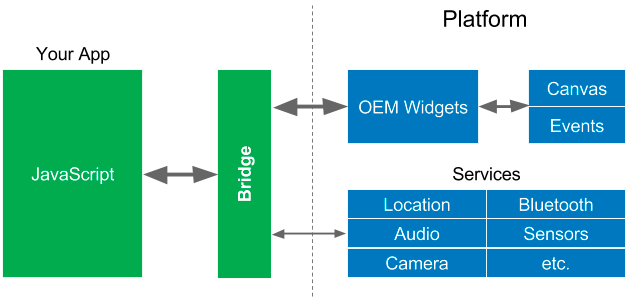
\includegraphics[width=7cm]{images/reactnative}
  \caption{Fonctionnement de React Native.}
  \label{fig:fonctionnement-rn}
\end{figure}

L’utilisation de composant natif permet des performances pratiquement identiques à celles des applications développées en code natif et évidement aucun chargement superflu est nécessaire. Une application écrite en React-Native ne dépend pas de la connexion internet de l’utilisateur, le code écrit avec React Natif est interprété en composant natif comme expliqué précédemment, il est donc possible de développer une application offline et donc limite les connections superflues contrairement aux applications hybrides qui sont totalement dépendantes de la qualité du réseau.  Cette interprétation en composant natif permet à un utilisateur iOS ou Android de retrouver un design cohérent entre l’application et le reste de son OS ou de ses autres applications téléchargées, il ne sera pas perdu en naviguant dans l’application, puisqu’il retrouvera l’ergonomie à laquelle il est habitué.
Contrairement aux applications hybrides, il ne s’agit pas d’une solution compatible à cent pourçent entre les différentes plateformes. Malgré cela, il est possible d'ajouter du code spécifique aux différentes plateformes en cas de besoin spécifique. Par exemple, l’application Instagram partage 85 \%  de code commun entre Android et iOS, le reste du code est spécifique à chaque plateforme. Heureusement, lors du développement React Native propose de compiler en fonction de la plateforme cible permettant de tester rapidement la compatibilité de l'application et d'avoir un code entièrement compatible et partagé entre Android et iOS. Facebook n’est pas seul pour mettre à jour son Framework, puisque plus de la moitié des nouvelles contributions sont ajoutées en Open Source par la communauté. Cette proportion particulièrement élevée indique une communauté particulièrement active. Les mises à jour sont donc plus fréquentes, et les réponses beaucoup plus rapides lorsqu’un développeur se retrouve bloqué sur une fonctionnalité de son projet.Cette communauté met au point de  très nombreuses librairies telles que Native Base ou React Native Element qu'il est possible d'ajouter rapidement à un projet existant pour étendre les composants disponibles de base.

 

Développé par Facebook depuis début 2015 et bénéficiant d’une large communauté, React Native continue d’évoluer avec le soutien de nombreux contributeurs sur Github. React Native est une technologie très prometteuse avec un énorme potentiel, qui a déjà été dûment appréciée par des géants comme Airbnb, Baidu, Discovery, Instagram et d’autres. Constamment améliorée et mise à jour par ses fondateurs, je pense qu'il s'agit d'une alternative à part entière à Objective C, Swift et Java.
 

\begin{figure}[htp]
  \centering
  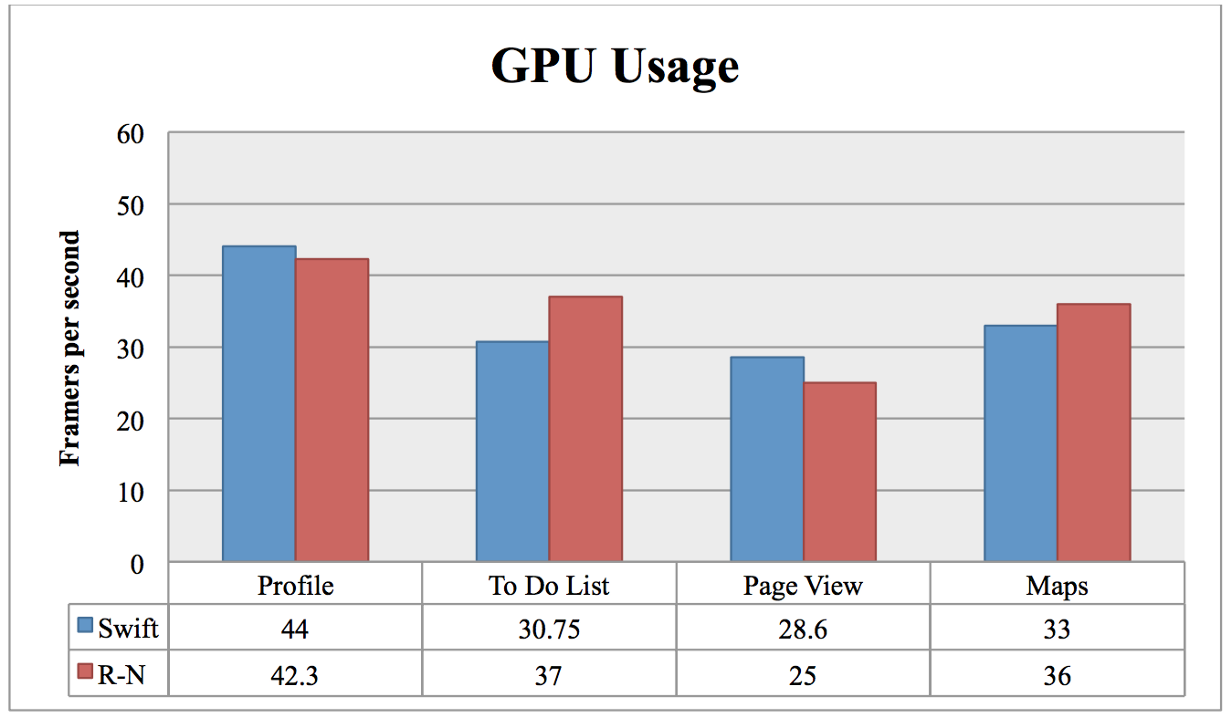
\includegraphics[width=7cm]{images/GPUusage}
  \caption{Différence de performance entre React Native et swift.}
  \label{fig:performance}
\end{figure}

En résumé, j'ai choisi de développer l'application mobile pour le système de recommandation d'articles en React Native. À la vue des contraintes de temps, de réactivité, d'évolutivité et du maintien de l’application. Pour moi il s'agit d'un bon compromis entre les applications natives et les applications composé uniquement de WebView.  


\section{Environnement de travail}

Dès le début de mon stage, le LRI m'as prêté un ordinateur portable sous Windows 10 pour travailler. De plus, j’ai mon téléphone personnel, un iPhone pour tester mon application mobile tout au long du développement, J’ai adapté mes choix logiciels en fonction de mes besoins pour ce stage.  

\subsection{IDE}

Visual Studio Code est un éditeur de code source développé par Microsoft pour Windows, Linux et OS X. Il est gratuit, open-source et inclut la prise en charge du débogage ainsi que le contrôle Git embarquer. Les fonctionnalités que Visual Studio Code contient sont prêtes à l'emploi mais il est possible d'ajouter des extensions en fonctions de ses besoins via un marketplace. Les extensions VS Code permettent d'ajouter la prise en charge des langages, des débogueurs. Pour mon travail sur React-Native,  j'ai installé comme première extension React Native Tools. Cette extension permet d'ajouter un environnement de développement spécifique à React Native. En utilisant cette extension, il est possible de lancer les commandes React-Native depuis la palette de commande VS Code et ajoute l’auto-complétions pour les APIs de React Native. Une seconde extension nommée Setup ESLint qui est un outil permettant d’améliorer la qualité du code JavaScript. Ce langage étant très permissif, il est très simple de glisser facilement sur du code illisible par un autre collaborateur. Eslint permet de structurer le code de façon uniforme. Tous les développeurs devront alors suivre les règles, le code est ainsi plus lisible. Dans le cas d'un développeur isolé comme durant mon stage, EsLint m’aide beaucoup à maintenir un code propre et uniforme.

\subsection{Gestion de version}

Un gestionnaire de version est un système qui enregistre l'évolution d'un fichier ou d'un ensemble de fichiers au cours du temps de manière à ce que l’on puisse rappeler une version antérieure d'un fichier à tout moment. Pour le développement de mon application, j'ai choisi d'utiliser Github. Github, c’est quoi ? Le nom GitHub est composé du mot « git » faisant référence au système de contrôle de version open-source et le mot « hub » faisant référence au réseau social bâti autour du système Git. Comme son nom ne l’indique pas, Github est un logiciel de gestion de version, mais pas que. C’est aussi un outil de développement collaboratif. GitHub est centré vers l'aspect social du développement. C’est le plus grand espace de stockage de travaux collaboratifs au monde. En plus d'offrir l'hébergement de projets avec Git, le site offre de nombreuses fonctionnalités habituellement retrouvées sur les réseaux sociaux comme les flux, la possibilité de suivre des personnes ou des projets ainsi que des graphes de réseaux pour les dépôts. Pour notre application, j’ai utilisé deux branches : Master et Dev permettant d’avoir une version de l’application fonctionnelle sur la branche Master et le travail en cours sur le développement de fonctionnalité ou correction de bug est faite sur la branche Dev. Au bout de chaque grande étape réalisée de l’application, une release est mise en place.

\subsection{Le SDK : expo.io}

Expo.io est un outil qui va nous permettre de développer une application avec React-Native et de se passer de XCode ou d’Android Studio. En implémentant le SDK expo dès la création du projet cela va me permettre de faire complétement abstraction de la plateforme de développement (iOS ou Android) ce qui rend ce projet plus « portable » qu’avec un projet purement en JS/React. Expo.io répond surtout à un besoin primaire de développement, je travaille sous Windows et je possède un iPhone. Je peux tester l’application que je développe sur Android via un émulateur fourni lors de l’installation d’Android Studio (l’IDE permettant de créer une application Android native) et normalement pour lancer une application sur un smartphone iOS (émulateur ou un smartphone), il est obligatoire de posséder un mac. Expo.io va me permettre de contourner cette contrainte. 

La principale particularité d'expo est de posséder un client disponible sur Android/iOS permettant de créer un tunnel entre l'application et le serveur expo sur mon ordinateur. Ce tunnel me permet le développement en local avec un déploiement distant (via l’application Expo sur Android/iOS) ce qui permet de pouvoir développer une application et de voir les modifications instantanément sur mon smartphone iOS sans posséder un mac. 

Mis à part les outils de développement, Expo.io fourni le format de fichier nécessaire pour le téléchargement de l’application dans les deux magasins d'applications, et le processus est relativement facile à faire. Ce SDK offre également des composants supplémentaires et avancés permettant d'accéder plus rapidement telles qu'un accéléromètre par exemple et pleinement compatible Android/iOS, utilisant ce SDK je suis certain de ne pas devoir créer du code spécifique à chacune des deux plateformes.




%%% Local Variables: 
%%% mode: latex
%%% TeX-master: "lri-report"
%%% End: 
\chapter{Realisation et implementation de l'application mobile}
\label{sec:Realisation de l'application mobile}

\section{Renewal}

\subsection{Les systèmes de recommandation}
Les systèmes de recommandation sont une forme spécifique de filtrage de l'information (SI) visant à présenter les éléments d'informations (films, musiques, livres, news, images, pages Web, etc) qui sont susceptibles d'intéresser l'utilisateur. Généralement, un système de recommandation permet de comparer le profil d'un utilisateur à certaines caractéristiques de référence et cherche à prédire l'« avis » que donnerait un utilisateur. Ces caractéristiques peuvent provenir de:

\begin{itemize}
    \item l'objet lui-même, on parle « d'approche basée sur le contenu » ou content-based approach. 
     \item L'utilisateur. 
    \item  l'environnement social, on parle d'approche de filtrage collaboratif ou collaborative filtering.

\end{itemize}

\subsection{Concurrence et la solution renewal}
Les recherches dans le domaine des systèmes de recommandation s’appuient la plupart du temps sur des évaluations “offline” qui ne permettent pas d’établir des métriques en phase avec une réelle satisfaction utilisateur. Dans le sous-domaine de la recommandation d’articles d’actualité, il existe à ce jour très peu de système permettant aux différentes équipes de recherche de tester leurs algorithmes en temps réel, i.e. sur des utilisateurs interagissant directement avec le système de recommandation.


La NewsREEL Live Task \cite{clef-newsreel} est, à notre connaissance, le seul système permettant de confronter différentes équipes sur des données en temps réel. Cependant, ce système est contraint sur plusieurs plans :

\begin{itemize}
    \item les données et le tracking des utilisateurs sont limités et ne permettent pas des recommandations à long terme. 
    
    \item  il n’existe pas d’interface dédiée à la recommandation et proposant des articles provenant de différentes sources.

\end{itemize}

Le projet Renewal se concrétise par le développement d'une application qui devra permettre de contourner les contraintes citées pour NewsReel Live Task et de permettre l'évaluation de nos algorithmes de recommandation sur des utilisateurs en contexte et en temps réel. Par la suite, nous proposons de développer un système qui tentera de contourner ces obstacles, ce qui aménera à la confrontation de différentes équipes de recherche. L'ensemble de ces contraintes énoncées doivent être prise en compte dès le début du développement de l'application mobile.


\subsection{Le concept Renewal}

Le concept central est construit autour de 2 types de recommandations au sein d'une application mobile dédiée. Ce contexte permet une analyse riche et fine du comportement avec un large panel d’indice conceptuel comme la géolocalisation ou le niveau de batterie sur le long terme. La tâche principale de Renewal est de recommandées des nouvelles diverses recommandé spécifiquement pour un utilisateur donné. La liste d’article générée pour l’utilisateur est le fruit de deux systèmes de recommandation que nous appellerons A et B. Lorsque l’utilisateur fait défiler les articles ou choisi un article, le moindre mouvement dans sa navigation est finement analysé via le temps, la vitesse de défilement, le temps de lecture du titre et bien plus. L’analyse fine du comportement permet de connaitre si l’algorithme A est plus pertinent que l’algorithme B ou inversement et de remplacer l’algorithme le moins pertinent par un algorithme C. Cette compétition permettra de connaitre in fine le meilleur algorithme de recommandation dans le sous domaine de la recommandation d’article. Une tache secondaire mais extrêmement importante est la recommandation d’article complémentaire non redondant avec la liste d’article recommandée via la recommandation diverse et surtout de fournir des informations supplémentaires sur un article donné. La navigation d’articles complémentaires est imaginée comme un parcours d’article en article sous forme arborescente. 

\begin{figure}[htp]
  \centering
  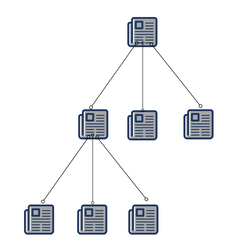
\includegraphics[width=7cm]{images/arbo}
  \caption{Methode arborescente}
  \label{fig:arbo}
\end{figure}


Renewal se veut être une plateforme modulaire où diverse équipe de recherche pourront proposer leur algorithme de recommandation d’article selon un contexte extrêmement riche et une base importante d’utilisateur. Cette expérience permettra aux équipes de recherches d’obtenir des statiques extrêmement complètes sur le résultat produit par leur algorithme à grande échelle.  


\section{Accès et analyse du comportement de l'utilisateur}

\subsection{User Cold Start}

En l’absence totale d’information sur l’utilisateur, la seule solution adoptée est d’utiliser des données externes, typiquement en s’aidant des informations sur les réseaux sociaux, c’est la direction que nous avons choisi pour l’application en accord avec la thèse préparée par Julien HAY. D’autres techniques s’appuient sur des méthodes spécifiques lorsque peu de données sont présentes, une review de ces méthodes est détaillée dans Dealing with the new user cold-start problem in recommender systems: A comparative review de Le Hoang So

L’idée est d’exploiter les posts et partages dans la recommandation pour résoudre la problématique du user cold start. Dans nos expérimentations, nous allons modéliser chaque type de contenu et chaque type d’interaction (partage, retweet, tweet, citation...) selon différentes pondérations et créer un vecteur représentatif des utilisateurs en utilisant des techniques de text embedding conditionnées par les triplets user-interaction-content. Nous appuierons nos travaux sur l’article Analyzing user modeling on Twitter for personalized news recommendations (2011) \cite{Analyzing} qui prend en compte les posts utilisateurs dans de la news recommendation et Improving User Topic Interest Profiles by Behavior Factorization (2015) \cite{User} qui séparent le contenu par type d’interaction.



\subsection{Gestion du compte utilisateur}

Au sein de notre application, nous avons choisi de laisser le choix à l'utilisateur d'utiliser soit une simple inscription par mail soit via un réseaux social. L'inscription via un simple mail rend plus complexe l'analyse des recommandations puisque nous avons aucune information complémentaire permettant de recommander des articles pertinents pour ce dernier. Au contraire, la connexion via Google, Facebook et Twitter permet selon les droits accordés à notre application Renewal de disposer de plus d'information concernant notre futur utilisateur. Ce type de connexion est de plus en plus plébiscité par les utilisateurs dont l'inscription à un contenu s'effectue en quelque seconde sans avoir besoin de rentrer son adresse mail et son mot de passe dans la plupart des cas où l'utilisateur est soit déjà connecté sur ce réseau ou dispose de l'application sur son smartphone.

\subsection{Evaluation du comportement et de la pertinance au sein de la recommandation}

Pour connaitre si un article est pertinent pour un utilisateur il faut étudier finement le comportement de l'utilisateur au sein de l'application. Dans un premier temps sur la liste d'article recommandé à l'utilisateur, il faut connaitre le temps passé sur la liste et les articles visibles pour l'utilisateur et à combien de pourcent. Si l’utilisateur passe un moment à regarder l’image et le titre de l’article ou au contraire il sélectionne très rapidement un article.

\begin{figure}[htp]
  \centering
  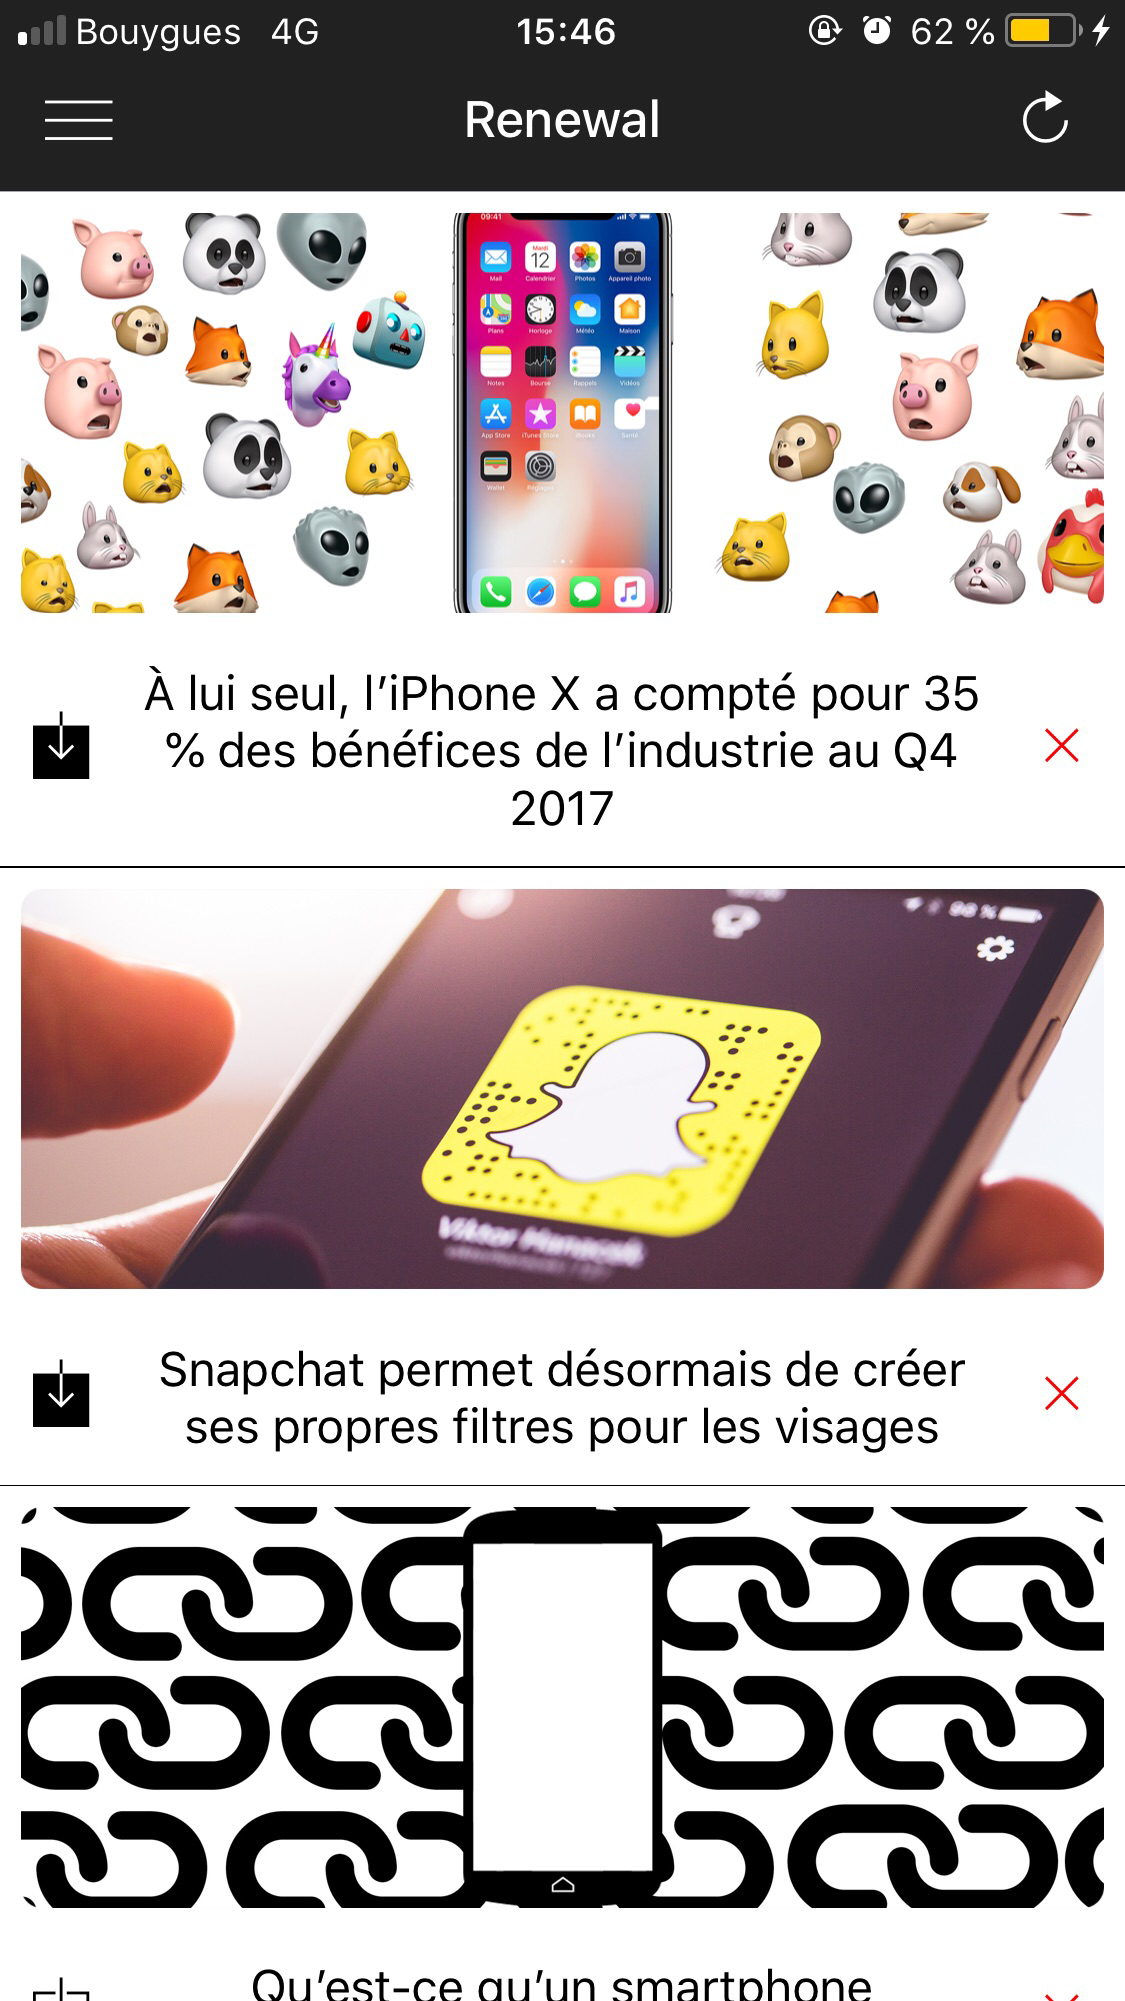
\includegraphics[width=7cm]{images/divers}
  \caption{Exemple de recommandation diverse.}
  \label{fig:screen-settings}
\end{figure}


Pour analyser le plus finement possible le comportement de l’utilisateur, il faut obtenir le maximum d’informations sur sa navigation et les conditions selon lequel il utilise l’application.  La récolte d’information peut s’effectuer via les différents capteurs disponibles sur le smartphone comme l’accéléromètre ou la localisation de l’individu nous permettant de proposer des actualités locales à l’utilisateur et de déterminer ses habitudes. La navigation au sein de la liste d’articles recommandés, notamment les articles visibles par l’utilisateur et à combien de pourcentage sont-ils visibles permet de savoir si la vignette de l’article, le titre de l’article ou les deux ont le plus d’importance pour l’utilisateur.  La détermination du temps passée sur la liste à son importance pour la détermination des articles recommandés.  
La récolte du plus d’information possible par utilisateur est extrêmement important pour les équipes de recherche et les capteurs permettent de savoir si l'utilisateur marche ou est simplement en mouvement. Les personnes en mouvement sont potentiellement susceptible de cliquer sur une vignette aguicheuse d’un article plutôt qu’un titre ou inversement cela sera déterminé par les équipes de recherche et leurs algorithmes de recommandation. La lecture d’un article sera aussi très finement analysée permettant de vérifier la pertinence de l’article via le temps passé à lire l’article ou si l’utilisateur à partagé l’article à un ami. En effet, si l’utilisateur reste 10 secondes sur l’article ce dernier n’est surement pas pertinent pour l’utilisateur.



\subsection{Loi RGPD}

Le Règlement général sur la protection des données (RGPD ou GDPR, pour General data protection régulation en anglais) est le nouveau cadre européen concernant le traitement et la circulation des données à caractère personnel, ces informations sur lesquelles les entreprises s’appuient pour proposer des services et des produits. Avant le RGPD existait une directive sur la protection des données personnelles qui date de 1995. Ce texte est abrogé par le RGPD. Le déploiement du RGPD dans l’espace européen se fait en deux temps : il y a d’abord eu, le 14 avril 2016, l’adoption définitive du texte par le Parlement. Cependant, son application ne s’est pas déroulée au même moment : il a été décidé de la décaler de deux ans, au 25 mai 2018 soit 2 mois après le début de mon stage. 


Du point de vue de l’internaute, le RGPD met en place ou conforte un certain nombre de protections. Il faut par exemple que les entreprises récoltent au préalable un consentement écrit, clair et explicite de l’internaute avant tout traitement de données personnelles, ou qu’ils s’assurent que les enfants en-dessous d’un certain âge aient bien reçu l’aval de leurs parents avant de s’inscrire sur un réseau social.

Le RGPD inclut aussi une reconnaissance d’un droit à l’oubli pour obtenir le retrait ou l’effacement de données personnelles en cas d’atteinte à la vie privée, le droit à la portabilité des données, pour pouvoir passer d’un réseau social à l’autre, d’un FAI à l’autre ou d’un site de streaming à l’autre sans perdre ses informations et le droit d’être informé en cas de piratage des données. Les internautes pourront aussi être défendus par les associations dans le cadre d’une action de groupe en vue de faire cesser la partie illicite d’un traitement de données.

Dans le cadre du développement de mon application mobile, j'ai exploité fortement les données issues des réseaux mais aussi l’analyse fine du comportement de l’utilisateur. Dans la loi RGPD, Facebook a durci l’accès aux données pour protéger ses utilisateurs. La rédaction d’un long dossier est nécessaire pour avoir accès à des données avancées (autre que le nom, prénom, email, date d’anniversaire) durant lequel il faut expliquer pour chaque donnée avancée l’utilisation faite par notre entreprise/application.  La rédaction de ce dossier permet à Facebook de s’assurer que notre application n’exploite pas les données de chaque utilisateur de façon abusive. Depuis l’entrée en vigueur de la loi RGPD, il est obligatoire de pouvoir laisser à chaque utilisateur l’accès ou non à chaque élément permettant le tracking d’un utilisateur et l’exploitation de ses données. Une autre notion obligatoire depuis la loi est de permettre à chaque utilisateur de récupérer l’ensemble des données rassemblées sur lui facilement.


\subsection{L'accès aux données sensibles et inconvéniants }

Pour avoir un système de recommandation pertinent, il est nécessaire d'avoir accès à certaine information dite sensible de l’utilisateur. Ces informations permettront aux algorithmes d'avoir un contexte pour chaque utilisateur permettant de déterminer si un article correspond plus ou moins à un utilisateur donné. Les données dites sensibles nous serons accessibles seulement via la connexion des différents réseaux sociaux faite par l'utilisateur. L'obtention des données autres que l’adresse et le nom d'utilisateur n'est pas obtenue via une connexion basique à l'aide d'un bouton sur notre application Renewal. 


Cet accès aux données sensibles est extrêmement complexe à obtenir et demande l'approbation du réseau pour chaque donnée de façon individuel. Certaine donnée extrêmement personnelle de l'utilisateur comme les posts du son mur Facebook demande l'élaborateur d'un dossier complet permettant de justifier l'accès aux données mais aussi le contexte global de l'application et la réelle utilité des données. Pour expliquer plus précisément ma démarche, je vais prendre pour exemple Facebook mais l'obtention des données sur les autres réseaux est sensiblement la même.


En première étape, il faut inscrire l’application sur la plateforme développeur du réseau social en renseignant les coordonnées du délégué à la protection des données (obligatoire depuis la loi RGPD) et des renseignements concernant l’application elle-même comme le domaine de l’application, son but, etc.  L’ensemble de ces renseignements fourni permettront d'obtenir un identifiant unique de l’application qui couplé à une clé secrète accordera par la suite une connexion à l'API. Pour pouvoir faire une connexion basique entre notre application et Facebook, il faut spécifier à partir de quelle plateforme l'utilisateur va se connecter. Dans notre cas, il s'agit d'Android et iOS, une clé secrète unique sera générée pour chaque plateforme et permettant de créer manuellement un bouton connexion avec Facebook ou si la connexion aboutie permettra de récupérer des informations basiques comme l'email, le nom d'usage et le prénom. Dans le contexte énoncé pour notre application, ce type de connexion est moyennement intéressante et ne permet pas de contrer le problème du User Cold Start.


La seconde étape est essentielle pour la viabilité de notre application et ainsi contourner le problème du User Cold Start. Cette étape consiste à obtenir l'accès via l'API Facebook d'obtention des données plus personnelles sur l'utilisateur permettant d'avoir des systèmes de recommandation pertinent et une expérience satisfaisante pour un utilisateur lambda. En fonction du type de données demandé, l'accès est plus ou moins facile à obtenir. Concrètement, connaitre la date de naissance ou le sexe de l'utilisateur est une donnée relativement simple à obtenir. Contrairement aux posts de l'utilisateur, le contenue "liker" par ce dernier ou les récents partages qui sont des données accessibles seulement pour une minorité d'entreprise cela est d'autant plus vrai depuis l'application de la loi RGPD. J'ai commencé par demandé l'accès aux données les moins contraignantes en termes d'accès par Facebook, la démarche est plutôt simpliste mais demande un long moment d'attention. Dans un premier temps, il faut spécifier dans quel cadre nous avons besoin de cette information, dans quel but et préciser avec exactitude à quel moment l’appel à ce type de donnée intervient et quel sont les changements pour l'utilisateur. Facebook peu alors procéder à la vérification du dossier et tester l’exécution des faits énoncés manuellement par un opérateur habilité. Il faut aussi fournir les exécutables de l'application ici le  .apk ou .ipa de l’application ainsi qu’une courte vidéo explicative permettant d'aider Facebook à reproduire avec exactitude le moment où l’appel aux données est nécessaire. La validation par Facebook étant au cas par cas non automatisée. La démarche peut prendre plusieurs semaines avant d’obtenir l’approbation ou le refus de Facebook auquel cas il faudra recommencer entièrement la seconde étape.


\subsection{Gestion des paramètres de l'application}

\begin{figure}[htp]
  \centering
  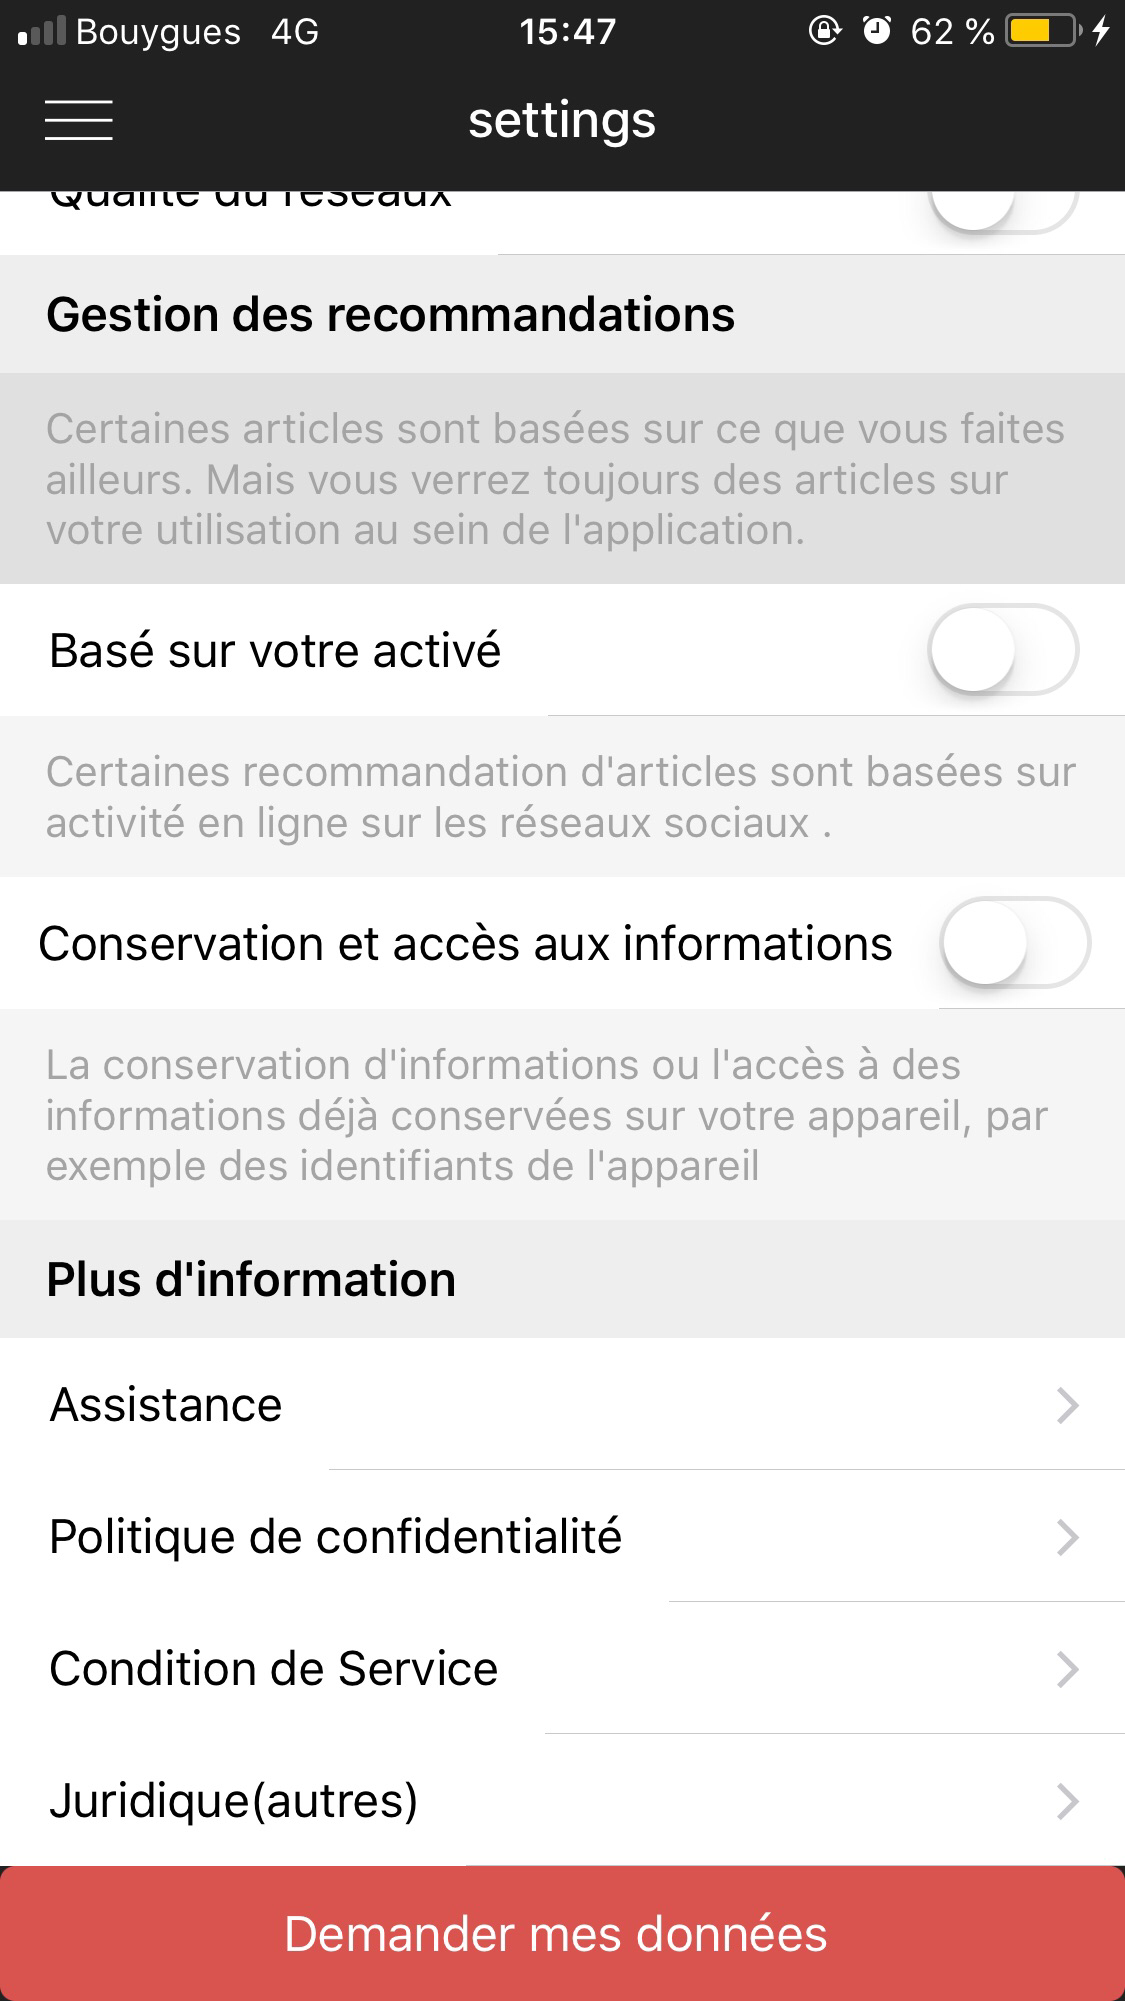
\includegraphics[height=10cm]{images/s2}
  \caption{Page des paramètres.}
  \label{fig:screen-settings}
\end{figure}

Depuis l'application de la loi RGPD, il est nécessaire d'offrir à l'utilisateur un droit de regard sur la gestion fine de ses données et d'expliquer dans quel but nous récoltons une information. Nous avons divisé la page de paramètres en trois sections :

\begin{itemize}
    \item La gestion des différents capteurs, permettant entre autres de connaitre la position de l’utilisateur et donc pour apporter plus d'informations contextuelles aux algorithmes de recommandation. 
     \item La gestion des recommandations, dans cette section permet de modifier l'accès aux données sur ses différents réseaux, ainsi que la conservation des données et le ciblage. 
    \item La section assistance et condition de service permettant à l'utilisateur d'obtenir plus d'informations sur l'application, son contexte et aussi de rentrer directement en contact avec l'équipe en charge du projet.

\end{itemize}




En bas de la page paramètres est disposé un bouton "Demander mes données" lui-aussi essentiel depuis la loi RGPD qui permet évidement l'envoi de l'ensemble des données récolté et stocké sur l'utilisateur depuis son inscription sur l'application Renewal. 

\section{Lecture d'un article}

\subsection{Analyse du comportement au sein d'un article}

Lorsqu'un utilisateur sélectionne un article, celui-ci est lancé dans une WebView. Nous avons fait le choix d'une WebView plutôt que l'extraction du contenue d'un article pour que l'utilisateur ne perde pas d'informations lors de la lecture d'un article puisque c'est le site dont l’article est issu donc l'information n'est pas détériorée ou coupée. L'utilisateur dispose donc un accès complet à l'article souhaité.

\begin{figure}[htp]
  \centering
  
\includegraphics[height=10cm]{images/webview}
  \caption{Exemple de WebView avec la languette.}
  \label{fig:screen-wv}
\end{figure}

La page de lecture est donc composée de deux éléments principaux mais aussi d'un composant crée par nos soins qui est "languette". La mise en place d'une WebView est aisée mais la communication entre notre application et la WebView fut compliquée à mettre en place. Notre WebView permet l'injection de JavaScript lors de l'exécution de la page. Le but est d'extraire un maximum d'information sur le comportement lors de la lecture d'un article comme le temps de lecture ou si l'utilisateur à parcouru l'ensemble de l'article. Pour les équipes de recherche, ces informations précieuses permettent de connaitre la pertinence de l'article vis à vis de cet utilisateur. Pour envoyer l'ensemble des informations regroupées dans la WebView à notre application j'utilise la fonction postMessage. Malheureusement toutes les fonctions relatives à l'envoi de message ne fonctionnent absolument pas et fait d'ailleurs l'objet de nombreuses issues sur le GitHub de React-Native. Face à ce problème deux solutions sont possibles la WebView va envoyer les paquets de données récoltées elle-même à un serveur, soit trouver une solution pour laisser l'application comme unique agrégateur de paquet. La première solution pose énormément de contrainte coté serveur comme faire concorder les flux en provenance de l'application et de la webView mais aussi donner à la WebView les moyens de se connecter au serveur. J'ai donc décidé de trouver une solution et contourner ce problème. A l'aide de la communauté GitHub, j'ai réussi à mettre en place un bridge dans l'envoi de message au sein de l'injection JS permettant l'envoi de données sous le format JSON. Une adaptation du code permettant la réception des messages a été nécessaire pour adapter la réception au format JSON. Cette étape à retardé la finalisation d'une semaine, le temps nécessaire à l'élaboration d'une solution viable. Aujourd'hui, cette solution est parfaitement fonctionnelle mais a nécessité l'ajout d'un tag afin de différencier les messages en provenance de notre analyse du comportement et ceux de certains sites.



Concernant la "languette", il s'agit d'un élément essentiel de notre application puisque la recommandation d'article complémentaire est faite à l'intérieur de cette languette. Le design final de la languette est le fruit d'une certaine réflexion. Il faut rendre cet élément non-intrusif lors de la lecture d'un article tout en insistant l'utilisateur à la découvrir. Nous avons choisi de minimiser au maximum l'espace pris par la languette à condition que celle-ci soit toujours swipable facilement. Une icone de flèche perpétuellement en mouvement indique à l'utilisateur la présence continuelle de la languette. 

Au sein de la languette, des éléments permettent de noter manuellement la pertinence de l'article et agiront de pair avec l'analyse faite automatiquement. Un bouton partage est disponible avec un certain nombre d'élément prérempli lors de l'envoi d'un article par mail ou par les réseaux sociaux. Ces éléments permettent de mettre en avant notre application lors des partages et donc l'augmentation de notre base d'utilisateur. Mais l'élément le plus important pour les équipes de recherche travaillant dans les systèmes de recommandation c'est la mise à disposition d'une liste d'articles complémentaires.


\subsection{La recommandation d'articles complementaires}


La tâche consiste à recommander des éléments d'actualités complémentaires à l'article actuel. Cette tâche est assez complexe puisque les articles proposés dans cette liste doivent apporter des informations complémentaires sans être redondant avec l'article actuel. De plus cette recommandation n'est pas considérée comme un élément secondaire de l'application mais un élément essentiel. D'un point de vue technique, la recommandation d'article complémentaire est imaginée comme une structure d'arborescence dans lequel l'utilisateur navigue d'articles en articles complémentaires et revient à la recommandation diverse une fois qu'il est suffisamment informé sur un sujet. Cette recommandation d'articles est un exercice complémentaire à la recommandation d'articles divers sur lequel les équipes de recherche seront mis aussi en compétition sur la pertinence et l'efficacité de leur algorithme.

\begin{figure}[htp]
  \centering
  
\includegraphics[width=7cm]{images/comp}
  \caption{Exemple de  recommandation de complementaire.}
  \label{fig:screen-comple}
\end{figure}

%%% Local Variables: 
%%% mode: latex
%%% TeX-master: "lri-report"
%%% End: 
\chapter{Amélioration technique de RENEWAL}
\label{sec:Amélioration technique de RENEWAL}

\section{Analyse ergonomique}

L'ensemble des écrans de l'application ont été réfléchi pour rendre l'expérience le plus naturel possible. Le nombre d'article de la liste de recommandation s'adapte à la taille de l'écran pour afficher le maximum d'article tout en gardant une bonne visibilité. A l'avenir, l'application sera disponible sur tablette et iPad, une de nos pistes de réflexion est la séparation de l'écran en deux lorsqu'une tablette est en orientation paysage. A gauche, sera disponible la liste d'article issus de la recommendation diverse et à droite la webview permettant la lecture d'un article.

Le code couleur, le style et la disposition actuel des éléments est le fruit d'une reflexion entre moi-même et J. HAY. Nous avons fait le choix de définir un style cohérent qui respecte l'ensemble des besoins énoncés au début du stage et lister dans le backlog de l'application. 

\section{Mise en favori d'un article}

Dans la liste d'article issu de la recommandation d'articles diverses, il est possible d'effectuer trois actions. Evidemment un clique sur l'article permet la lecture d'un article simplement. Une petite croix à droite du titre permet de griser l'article et donc d'exprimer clairement que l'utilisateur n'est pas satisfait de la recommendation de cet article. Une icone à gauche de l'article permet de mettre en favori un article. L'ensemble des articles mis en favoris sont regroupés au sein d'un écran disponible dans le menu latéral de l'application. Techniquement, les articles dans cette partie sont sauvegardés dans une base de donnée interne SQLite permettant à l'utilisateur de garder continuellement les articles mis en favoris et de trier les articles selon leur date de mise en favori. 

\section{Gestion de l'historique}

La partie historique est encore en reflexion, à l'avenir cette partie de l'application mettra en avant la structure arborescente des articles. L'idée est de regrouper l'historique par jour et par navigation d'article en article. Concrétement si à un jour X un utilisateur ne lit qu'un unique article, l'historique de cette journée ne montrera qu'un unique article. Mais si à un jour Y, l'utilisateur navigue d'articles complémentaires en articles complémentaires, l'historique de cette journée devra montrer la structure arborescente déssinée horizontalement. Cette partie de l'application, est en cours de reflexion, il faut prendre en compte la structure aborescente et la visibilité de cette structure. Dessiner un arbre au sein de l'application n'est pas une chose aisée et d'après mes recherches aucun membre de la communauté React-Native n'a tenté l'expérience.  

\section{La norme i18n}

L'internationalisation d'un logiciel (abrégé en i18n, où 18 représente le nombre de caractères entre le i et le n dans « internationalisation »), regroupe les bonnes pratiques en terme d'internationalisation et permettent aux développeurs et aux programmeurs de logiciels d'écrire des applications de meilleures qualités qui contribueront à une localisation ultérieure plus efficace.Et grâce à une gestion très précoce des questions d'internationalisation et de localisation au cours de la conception de logiciels. 

\section{La mise en avant du concept}

Lors de la première ouverture de l'application, il est nécessaire de montrer à l'utilisateur avec des mots simples le concept de Renewal. Le but étant de se distinguer des applications qui agissent seulement comme un agrégateur de contenu comme Google News par exemple et de mettre fortement en avant l'aspect recommandation d'article. Mais aussi faire comprendre à l'utilisateur qu'il est important pour nous et les équipes de recherche via leurs algorithmes de recommandations d'avoir un accès à minima à un de leurs réseaux sociaux. Pour la réalisation de cette partie, j'ai regardé comment les autres applications déjà installées sur un store expliquent leur concept comme notamment l'application Slack ou discord. Après une courte analyse, j'ai compris que pour avoir une information percutante il faut une image centrale avec juste un seul mot mis en avant. Ainsi, j'ai crée 3 pages, la première étant les remerciements adréssés à l'utilisateur pour avoir téléchargé l'application, la seconde mettant en avant le coté recommandations et la dernière page insitant l'utilisateur à se connecter via un réseau social avec le moyen d'ouvrir une page complémentaire permettant d'en savoir plus sur l'utilisation de ses données. 


%%% Local Variables: 
%%% mode: latex
%%% TeX-master: "lri-report"
%%% End: 
\chapter{React-Native et la compatibilité}
\label{sec:React-Native et la compatibilité}




\section{La compatibilité Android / iOS }


L’énorme avantage de React Native est l’insertion rapide de « module » externe développé par des tiers et souvent maintenu par la communauté très active de React Native sur GitHub. Le développement d’un module externe installable pour tout projet React Native demande de développer une partie du code spécifique à Android et à IOS. Au cours de mon développement, j’ai eu besoin de différents modules extrêmement spécifique, parfois le parfait module était disponible uniquement avec une des deux plateformes notamment parce que React Native est un Framework extrêmement jeune encore en version 0.55 et fait appel à des composants natifs de chaque plateforme. L’appel de différente fonction change encore régulièrement et une façon de procéder qui était valable il y a un an n’est parfois plus viable aujourd’hui. Certains modules non maintenus sont donc devenu inutilisable avec le temps. Ce changement de nomenclature est parfaitement compréhensible pour un Framework n’étant pas encore disponible en version 1 bien que parfaitement viable actuellement pour développer un large panel d’application donc les plus connues sont Uber, Skype ou Facebook. 
La majorité des modules développés par des tiers sont parfaitement compatibles avec Android et IOS, cependant je me suis souvent retrouvé face à des modules pour mon application qui étaient compatibles seulement avec IOS ou moins souvent avec des manipulations supplémentaires pour rendre le code compatible avec Android. Cependant, je me suis souvent retrouvé à devoir retravailler mon code pour faire fonctionner mon application sous Android. L’explication est simple, les appels des fonctions ou accès à des composants changent régulièrement d’une version d’Android à une autre. Une application développée en React-Native et le SDK expo.io offre énormément d’avantage mais la suppression des dossiers spécifiques à Android et IOS a eu certains inconveniants au cours de mon développement notamment celui de ne pas pouvoir insérer du code en Java pour Android par exemple. Ainsi, je ne pouvais faire que du code spécifique à chaque OS seulement en JavaScript et donc avec un impact limité par rapport à du code natif.  Je peux citer plusieurs exemples comme le stockage des données en local dont il m'a fallu tout changer pour rendre le code totalement asynchrone et compatible avec Android mais aussi le code du composant lié à la liste des articles dont l’évolution de React Native et Android à rendu incompatible. Testant spécifiquement le code développé sur un terminal IOS, j’ai tardé à tester mon application sur Android et donc le changement du composant lié à la liste d’articles est survenu tardivement et à entrainé du retard dans mon travail. Depuis cette erreur, j’ai compris que pour le développement d’une application cross-plateforme, il est nécessaire de pouvoir tester régulièrement l’application sur les différentes plateformes visées sous peine d’obtenir une dette technique qui s’accumule.  

\section{Publication de l'application}

Il est possible de partager notre projet publié via Expo Client et sur notre profil expo.io mais dans le cadre du projet Renewal il est nécessaire d'envoyer une application autonome aux magasins d'application d'Apple et de Google. La soumission à ces magasins implique des exigences et des normes de qualité plus élevées que le partage d'un projet avec d'autre développeur, car cela rend notre application disponible via une plateforme de distribution beaucoup plus large. Il est utile de jeter un coup d'œil sur les rejets communs d'applications. Les binaires peuvent être rejetés pour avoir des icônes mal formatées par exemple. Surtout dans le cas d'Apple où les règles d’acceptation changent régulièrement. L’ensemble des règles à respecter pour réussir la soumission d’une application sur l’Apple Store s’étoffe de plus en plus et à tendance à être fastidieuse et incohérente. Apple peut rejeter votre application si les éléments ne s'affichent pas correctement sur un iPad et même si votre application ne cible pas le forme factor de l'iPad. Expo ne peut pas garantir que notre projet sera accepté par l'une ou l'autre plateforme, et c’est à nous de mettre en conformité le comportement de notre application. Cependant, les applications Expo sont des applications natives et se comportent comme toutes les autres applications donc ne demande pas d'adaptation particulière. Par contre, Expo facilite la mise à jour de notre application, puisqu’il est possible de mettre à jour l’application dès son ouverture sans devoir mettre à jour l’application dans le magasin d’application. 





%%% Local Variables: 
%%% mode: latex
%%% TeX-master: "lri-report"
%%% End: 
\chapter*{Conclusion et perspectives}
\addcontentsline{toc}{chapter}{Conclusion}
\markboth{Conclusion}{Conclusion}
\label{sec:conclusion}

Ainsi, j’ai effectué mon stage de Master 1 MIAGE (Méthodes informatiques appliquées à la gestion des entreprises) au sein du Laboratoire de Recherche en Informatique. Faire partie d’une équipe dynamique, accueillante et compétente, m'a permis de travailler dans de bonnes conditions, d'appliquer mes connaissances acquises durant ma formation et d'en acquérir de nouvelles.  

 

Ma première mission durant ce stage fut le développement d'une application mobile.Ce travail s'est dérouler en plusieurs étapes : l'étude de la meilleure solution possible, le développement continu et la récupération des données utilisateurs.  

 

Ce projet représente pour moi une expérience notable au niveau de la programmation mobile. En effet, ces dernières années le marché des applications mobiles est en pleine croissance ainsi cette application arrive suite à ma formation sur la programmation mobile spécifique à Android dispensé au sein de mon cursus en Master 1 MIAGE me permettant de connaitre et de comprendre les problématiques liés à la programmation native et cross-plateforme. 
 

De plus, il est nécessaire de rappeler qu’à la date de rendu de ce rapport, mon stage n’est pas terminé. Me laissant le temps d'améliorer mon application mobile mais aussi de commencer le travail concernant la seconde mission qu'il m'a été attribuer au début de mon stage, c'est à dire la construction d'un système de recommandation baseline.

%%% Local Variables: 
%%% mode: latex
%%% TeX-master: "lri-report"
%%% End: 



\appendix

\bibliographystyle{authoryear-fr}
\bibliography{references}

\clearpage

%%%%%%%%%%%%%%%%
%%% Abstract %%%
%%%%%%%%%%%%%%%%

\thispagestyle{empty}

\vspace*{\fill}

\begin{center}
  Université Paris-Nanterre\\
  200 Avenue de la République\\
  92000 Nanterre
\end{center}
\vspace*{\fill}

\end{document}